\section{Methodology}
\label{sec:method}
In-context learning with few-shot prompting involves prompting a model with an instruction $\phi$ and $n$ demonstrations of input-output pairs $\mathcal{E} = \{(x_i, y_i)\}_{i=1}^n$, where $x_i \in X,\ y_i \in Y$. Here, $(x_i, y_i)$ denotes the input-output pair for the $i$-th demonstration, and $X$ and $Y$ refer to the sets of inputs and outputs, respectively. The model is expected to exploit the demonstrated examples to produce an output $y'$ for an unseen input $x'$. In the inductive reasoning variant of ICL, the model is prompted with a rule-generation instruction $\phi_{\mathrm{rg}}$ to learn a function $f: X \rightarrow Y$ that maps inputs to outputs. We refer to this step as the \emph{rule or hypothesis generation} step. Next, the model is prompted with an instruction $\phi_{\mathrm{rf}}$, the learned rule $f$, and an unseen input $x'$ to produce the output $y'$. We refer to this step as \emph{rule-following}. Our objective is to distill the inductive reasoning ability of a teacher model into a student model.

Some reasoning tasks, such as the 1D ARC task, are difficult for open-weight models, and prior works have therefore used large proprietary models such as GPT-4~\citep{wang2023hypothesis}. This prompted us to use GPT-4o as our teacher model. Using a proprietary model as a teacher poses challenges for using traditional distillation techniques that rely on output logits~\citep{hinton2015distillingknowledgeneuralnetwork} or intermediate representations~\citep{romero2015fitnetshintsdeepnets}. To mitigate this issue, we use a black-box distillation approach via data augmentation~\citep{li2022explanationslargelanguagemodels}. Our method has three steps: data augmentation using the teacher model, supervised fine-tuning, and preference alignment of the student model. An overview of this process is shown in Figure~\ref{fig:proposed_method}.

\begin{figure}
    \centering
    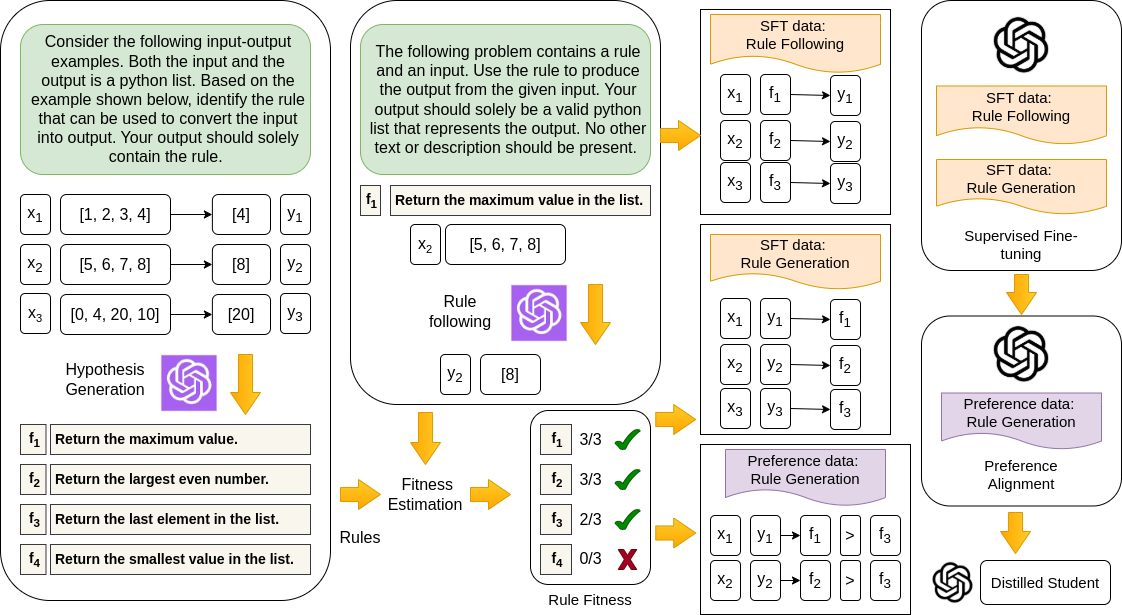
\includegraphics[width=\textwidth]{Figures/colm_2025_proposed.png}
    \caption{Overview of data augmentation, filtering and model tuning in \proposed. The teacher and student models are shown in purple and black, respectively. Each entry in the rule generation corpus contains multiple few-shot demonstrations. Each entry in the SFT and preference alignment corpora includes both the rule generation and the corresponding rule-following instructions. These details are omitted for clarity.}
    \label{fig:proposed_method}
    \vspace{-1em}
\end{figure}

\paragraph{Data augmentation} 
During data augmentation, we first use a set of in-context demonstrations, $\mathcal{E}$, to generate a set of $m$ hypotheses from the teacher model. Let $f_j$ be one candidate hypothesis. The next step is to use the teacher model to perform rule following and determine how well the examples in $\mathcal{E}$ align with $f_j$. Thus, a fitness score $s_j$ is computed for a candidate hypothesis $f_j$ as follows:
\begin{equation*}
    s_j = \sum_{i=1}^n [f_j(x_i) = y_i]
\end{equation*}
Since the teacher model's rule-following ability is imperfect, we refer to the process as noisy fitness estimation. After data augmentation, we perform quality analysis and filtering. We construct two separate datasets: one for supervised fine-tuning involving both rule following and rule generation, and another for preference alignment containing chosen and rejected rule pairs.

Let $T$ be the number of reasoning tasks in the ICL dataset. Let $\Gamma_{\mathrm{rg}}^{\mathrm{s}}$, $\Gamma_{\mathrm{rf}}^{\mathrm{s}}$, and $\Gamma_{\mathrm{rg}}^{\mathrm{p}}$ refer to the SFT dataset for rule generation, the SFT dataset for rule following, and the preference alignment dataset for rule generation, respectively. They are constructed as follows:
\begin{align*}
    \Gamma_{\mathrm{rg}}^{\mathrm{s}} &= \left\{ (\phi_{\mathrm{rg}}, \mathcal{E}^t, f_j^t) : s_j^t \geq \tfrac{n}{2} \right\}_{t=1}^T \\
    \Gamma_{\mathrm{rf}}^{\mathrm{s}} &= \left\{ (\phi_{\mathrm{rf}}, f_j^t, x_i^t, y_i^t) : s_j^t \geq \tfrac{n}{2},\; 1 \leq i \leq n \right\}_{t=1}^T \\
    \Gamma_{\mathrm{rg}}^{\mathrm{p}} &= \left\{ (\phi_{\mathrm{rg}}, \mathcal{E}^t, f_j^t, f_k^t) : 1 \leq j,k \leq m,\; s_j^t > s_k^t + d \right\}_{t=1}^T
\end{align*}
To ensure the high quality of the SFT datasets, we only allow hypotheses that satisfy at least half of the examples in $\mathcal{E}$. To check whether a hypothesis satisfies an example, we use the teacher model's rule-following ability with natural language. Since the teacher model may not perfectly follow rules, even a perfect hypothesis might not receive a perfect score. Setting the rule quality threshold to $50\%$ ensures that the high-quality rules remain in the dataset. For the preference dataset, we select all hypothesis pairs within a task such that the score difference between the chosen rule and the rejected rule is greater than a threshold $d$.

\paragraph{Supervised Fine-tuning} We perform supervised fine-tuning on the student model during the model tuning phase using low-rank adaptation. The SFT dataset comprises both rule generation and rule-following examples across all tasks. The goal is to maximize the likelihood $\log P(f_j \mid \phi_{\mathrm{rg}}, \mathcal{E})$ and $\log P(y_i \mid \phi_{\mathrm{rf}}, f_j, x_i)$ for rule generation and rule following, respectively.

\paragraph{Preference Alignment} 
After supervised fine-tuning, we perform preference alignment to improve the quality of rule generation within a smaller hypothesis search space. The best-performing alignment method, ORPO, is defined based on the odds ratio of generating the chosen hypothesis relative to the rejected hypothesis. Given an instruction $\phi_{\mathrm{rg}}$ and ICL demonstration $\mathcal{E}$, the odds of generating a hypothesis $f_j$ are defined as:
\begin{align*}
    \mathrm{odds}(f_j \mid \phi_{\mathrm{rg}}, \mathcal{E}) 
    &= \frac{P(f_j \mid \phi_{\mathrm{rg}}, \mathcal{E})}{1 - P(f_j \mid \phi_{\mathrm{rg}}, \mathcal{E})}
\end{align*}

The odds ratio of generating the chosen hypothesis $f_j$ relative to the rejected hypothesis $f_k$, and the associated loss function $\mathcal{L}_{\mathrm{or}}$, are as follows:
\begin{align*}
    \mathrm{odds\_ratio}(f_j, f_k) 
    &= \frac{\mathrm{odds}(f_j \mid \phi_{\mathrm{rg}}, \mathcal{E})}{\mathrm{odds}(f_k \mid \phi_{\mathrm{rg}}, \mathcal{E})} \\
    \mathcal{L}_{\mathrm{or}} 
    &= -\log \sigma\big( \log \mathrm{odds\_ratio}(f_j, f_k) \big)
\end{align*}

The overall preference alignment loss for ORPO is computed via a weighted combination of the SFT loss $\mathcal{L}_{\mathrm{sft}}$ and the odds ratio loss $\mathcal{L}_{\mathrm{or}}$:
\begin{align*}
    \mathcal{L} 
    &= \mathcal{L}_{\mathrm{sft}} + \lambda \mathcal{L}_{\mathrm{or}}
\end{align*}


